\section{Experiments}
\label{sec:experiments}

This section presents the results of applying our shape projection operators along with deep shape priors for
three reconstruction tasks.

\begin{figure*}
\centering
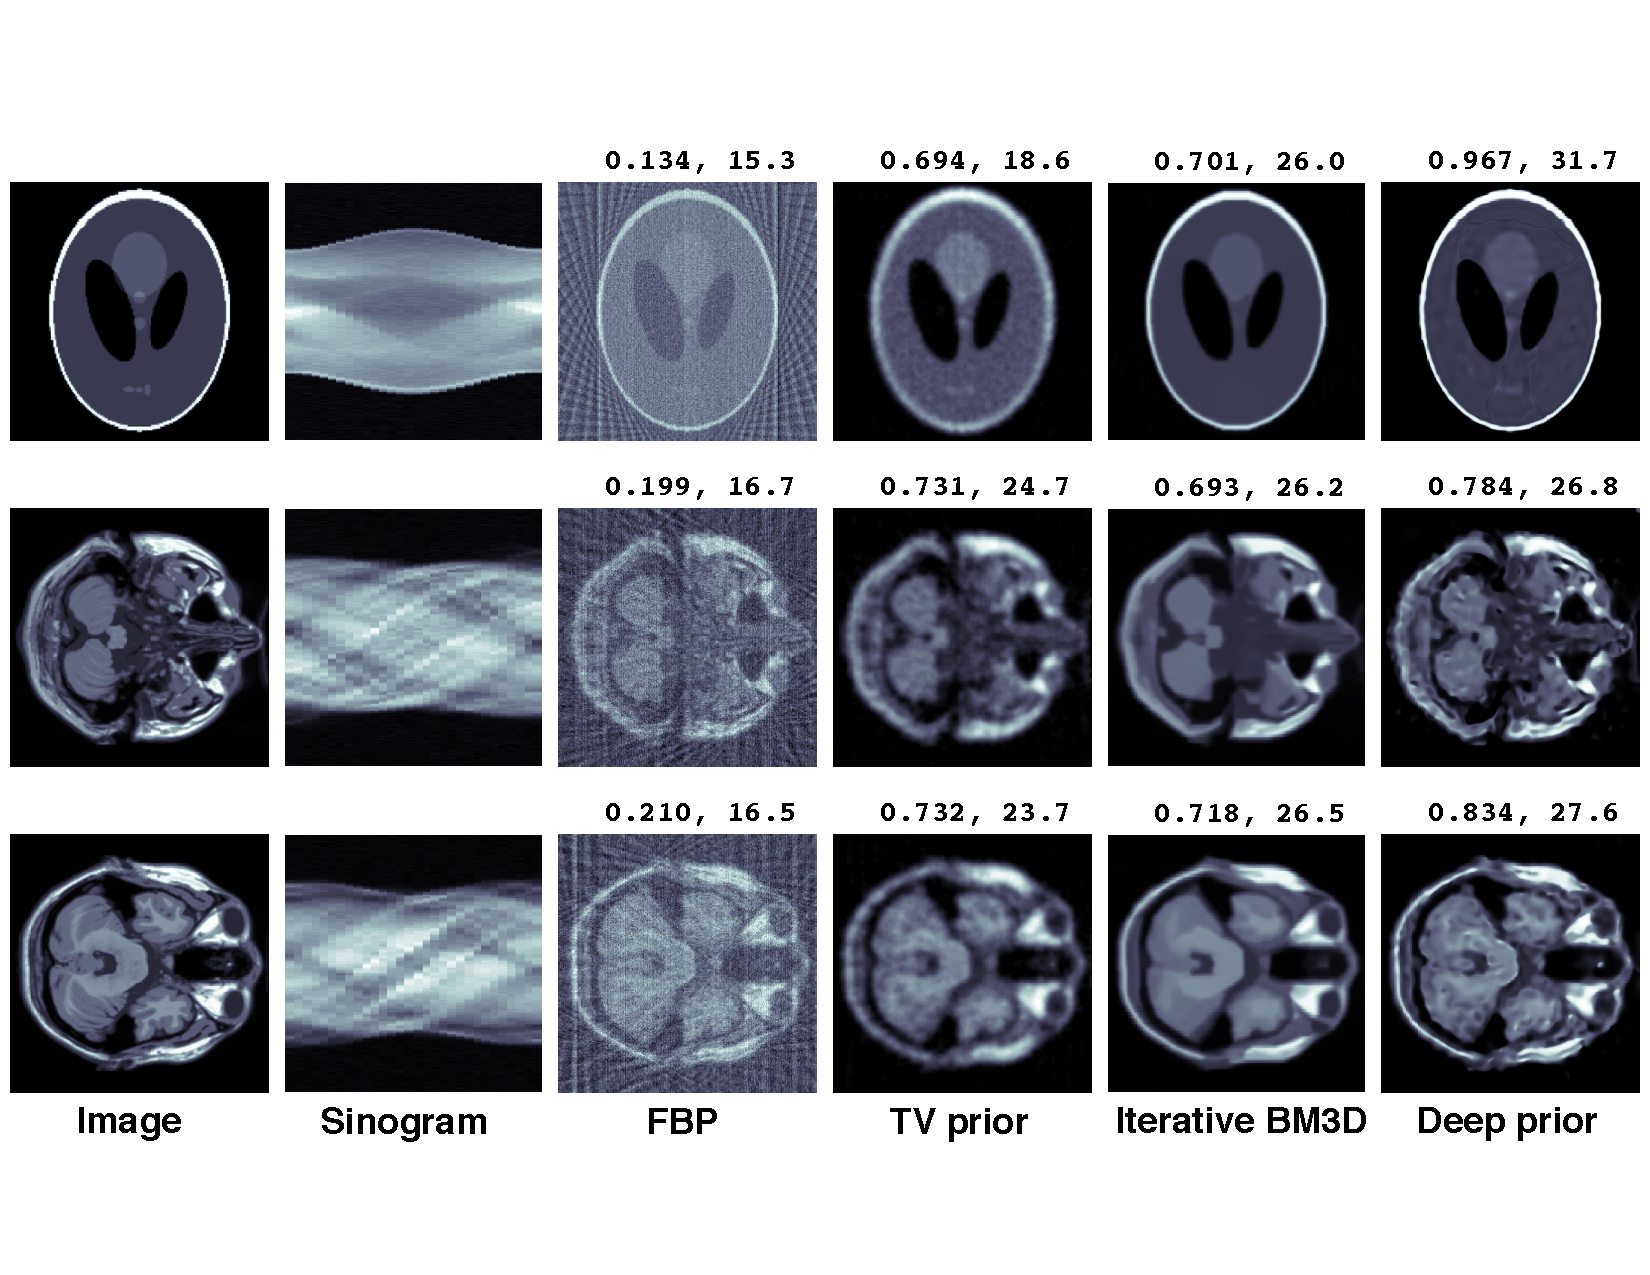
\includegraphics[width=\linewidth]{dsp/figs/CTcomparison-text.pdf}
\caption{\label{fig:ct} \textbf{Tomographic reconstruction
    results} from sinograms (radon transforms) sampled with $n = 30$
  angles and noise ($\sigma=1$). The sinogram is rescaled to the image
  size with nearest neighbor interpolation for visibility. From left
  to right in each row is the noise free image, the noisy sinogram,
  reconstruction with the filtered backprojection (FBP), TV prior,
  BM3D, and deep image prior. The SSIM and PSNR are shown for each
  approach on top of the corresponding figure. Our approach
  outperforms the other learning free baselines by a significant margin. \emph{Zoom in for details.}}
\end{figure*}

\paragraph*{Network Architecture.}
In the volumetric reconstruction experiments (i.e. reconstructing 3D shapes from silhouette images and depth images respectively), the network architecture is a fully convolutional UNet~\cite{ronneberger2015u} where the encoder 
has 5 layers with 8, 16, 32, 64 and 128 filters.
The decoder is a mirrored version of the encoder and skip connections are applied just in the 2 innermost layers.
The upsampling is done through bilinear/trilinear interpolation followed by a convolution.
All convolutions have filter size 3 and are followed by batch normalization and ReLU activation function.
The input to the network is a tensor of the same size as the output, and its values sampled from $\mathcal{N}(0,1)$. In all the experiments, we used Adam optimizer with learning rate=$10^{-2}$.

For the image reconstruction (i.e. tomography) we doubled the number of filters in each layer keeping the rest of the network architecture identical to account for higher spatial frequency of the underlying signal.
The only other difference between the network that produces images and the one that produces
voxel grids is that the convolutional operations are performed in 2D instead of 3D.
Even though the network can be used to generate data of any size (since it is fully convolutional),
in our experiments we set our image resolutions to $256\times256$ and voxel resolution to $128^3$.

\begin{figure*}[t]
\centering
\setlength{\tabcolsep}{0pt}
\begin{tabular}{c|cccc}
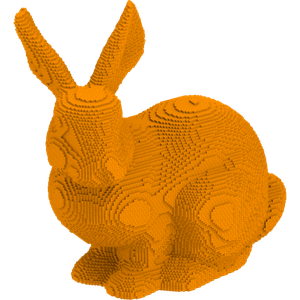
\includegraphics[width=.2\linewidth]{dsp/figs/gt.png} &
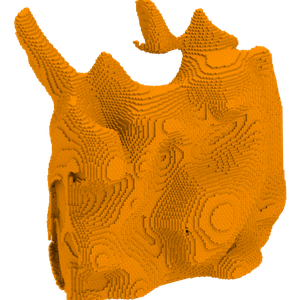
\includegraphics[width=.2\linewidth]{dsp/figs/bunny_deep_4binary.png} &
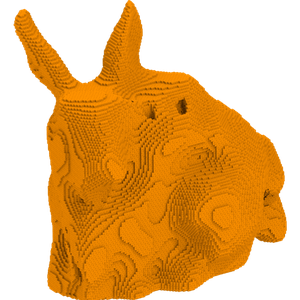
\includegraphics[width=.2\linewidth]{dsp/figs/bunny_deep_8binary.png} &
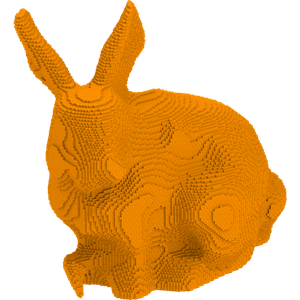
\includegraphics[width=.2\linewidth]{dsp/figs/bunny_deep_16binary.png} &
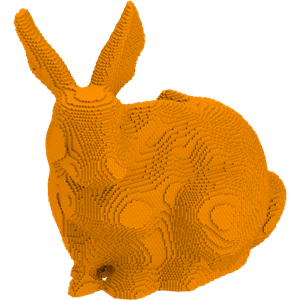
\includegraphics[width=.2\linewidth]{dsp/figs/bunny_deep_32binary.png}\\
GT &
4 views &
8 views&
16 views&
32 views
\end{tabular}
    \caption{\small \label{fig:binview} \textbf{Effect of the number of views in the reconstruction from silhouettes.}
		3D shape reconstructed from silhouette images of the same object.
		Even without having access to enough 3D information, our method is still capable of generating
		plausible shapes.
    }
\end{figure*}


\subsection{Tomography Reconstruction}
In tomographic reconstruction our goal is to invert the sinograms as described in Section~\ref{sec:method}.
With deep image prior the reconstruction involves solving the following optimization problem:
\begin{equation}
	\min_{\bm{\theta} \in \mathbb{R}^D} ||R - \mathcal{T}_R(f_{\bm{\theta}}(\bm{\eta}))||_1,
\end{equation}
where $f$ is our neural network described above, $\bm{\eta}$ is its noise input, and $R$ is the input sinogram (which may have low angular sampling rate and/or be corrupted by noise). To test the ability of our algorithm when handling challenging input, we use a low angular sample rate ($n=30$) and simulate noisy sinograms by adding a Gaussian noise of $\sigma=1$.
Figure~\ref{fig:ct} shows the reconstruction results of the Shepp-Logan phantom image~\cite{shepp1974fourier} and two separate slices of a sample from the BrainWeb database~\cite{cocosco1997brainweb}.
These images have been commonly used to evaluate CT reconstruction algorithms.
For each reconstruction we compute the structured similarity (SSIM) index and PSNR values with respect to the groundtruth image (higher is better).

The standard solution for tomography is Filtered Back Projection (FBP): it inverts the Radon transform using the Fourier slice theorem. When angular sampling rate is low, the reconstruction using FBP turns out to have severe aliasing artifacts as seen in Figure~\ref{fig:ct} third column.
The TV prior significantly improves the reconstructions for all three images.
The iterative BM3D approach~\cite{maggioni2013nonlocal} described in Section~\ref{sec:related} was run for 100 iterations. We noticed that the PSNR values converged after 100 iterations with the largest gains in PSNR in the first 20 iterations.
Note that running BM3D on the FBP reconstruction corresponds to one iteration of this approach.
For the deep prior we obtain results by running $2000$ gradient steps.
Compared to iterative BM3D, the deep prior produces reconstructions with significantly better SSIM values and comparable or better PSNR values (last two columns in Figure~\ref{fig:ct}).
The relatively poor performance of BM3D may be because the aliasing noise in CT reconstructions tends to be more structured and less like natural image noise when compared to the noise observed in image denoising applications.
It takes many iterations for the iterative BM3D algorithm to get rid of the artifacts produced by the inverse radon transform but this causes smoothing of the underlying structures leading to lower SSIM scores.

\subsection{Shape-from-Silhouette 3D Reconstruction}

\begin{figure*}[t]
\centering
\setlength{\tabcolsep}{0pt}
\begin{tabular}{cccccccc}
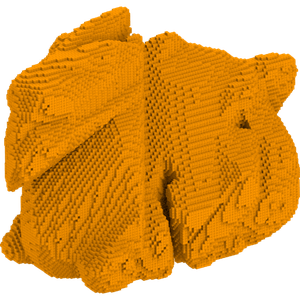
\includegraphics[width=.14\linewidth]{dsp/figs/dragon_carve_binary_8_0.png} &
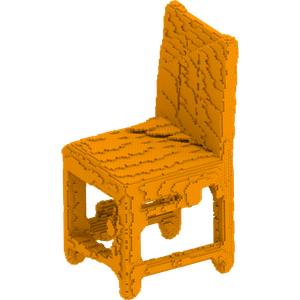
\includegraphics[width=.14\linewidth]{dsp/figs/chair_0013_carve_binary_8_0.png} &
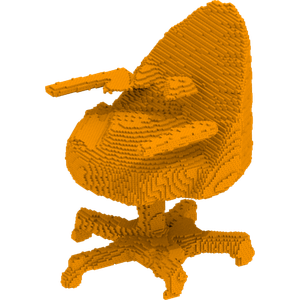
\includegraphics[width=.14\linewidth]{dsp/figs/chair_0200_carve_binary_8_0.png} &
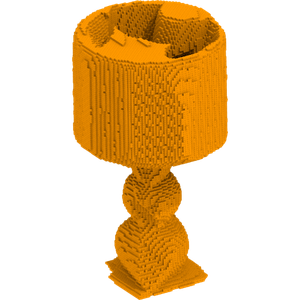
\includegraphics[width=.14\linewidth]{dsp/figs/lamp_0050_carve_binary_8_0.png} &
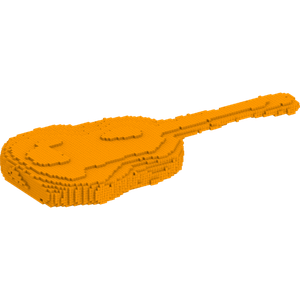
\includegraphics[width=.14\linewidth]{dsp/figs/guitar_0100_carve_binary_8_0.png} &
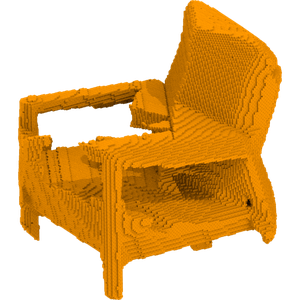
\includegraphics[width=.14\linewidth]{dsp/figs/chair_0011_carve_binary_8_0.png} &
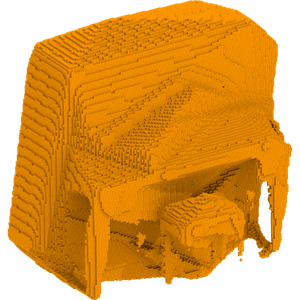
\includegraphics[width=.14\linewidth]{dsp/figs/piano_0050_carve_binary_8_0.png} \\

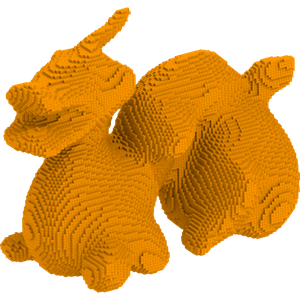
\includegraphics[width=.14\linewidth]{dsp/figs/dragon_deep_binary_8_0.png} &
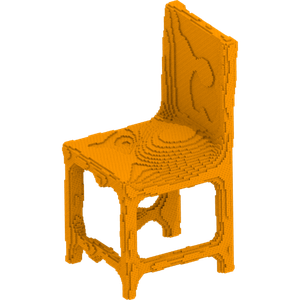
\includegraphics[width=.14\linewidth]{dsp/figs/chair_0013_deep_binary_8_0.png} &
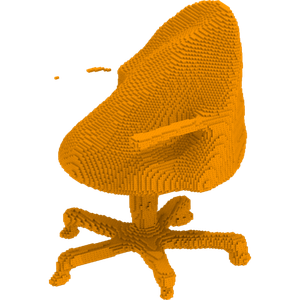
\includegraphics[width=.14\linewidth]{dsp/figs/chair_0200_deep_binary_8_0.png} &
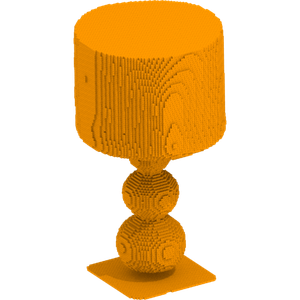
\includegraphics[width=.14\linewidth]{dsp/figs/lamp_0050_deep_binary_8_0.png} &
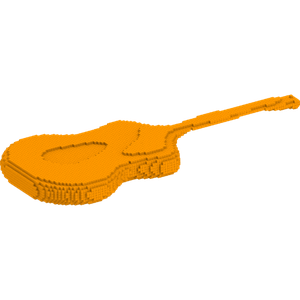
\includegraphics[width=.14\linewidth]{dsp/figs/guitar_0100_deep_binary_8_0.png} &
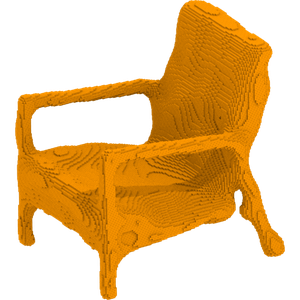
\includegraphics[width=.14\linewidth]{dsp/figs/chair_0011_deep_binary_8_0.png} &
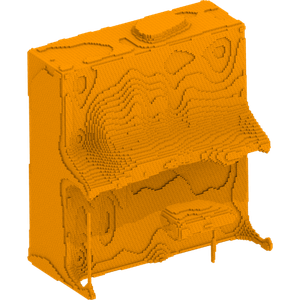
\includegraphics[width=.14\linewidth]{dsp/figs/piano_0050_deep_binary_8_0.png} \\

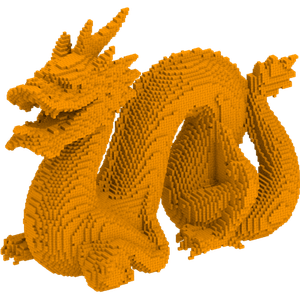
\includegraphics[width=.14\linewidth]{dsp/figs/dragon.png} &
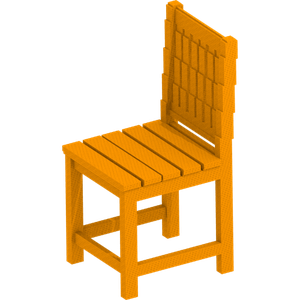
\includegraphics[width=.14\linewidth]{dsp/figs/chair_0013} &
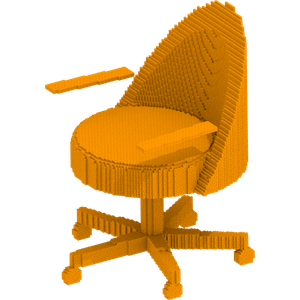
\includegraphics[width=.14\linewidth]{dsp/figs/chair_0200.png} &
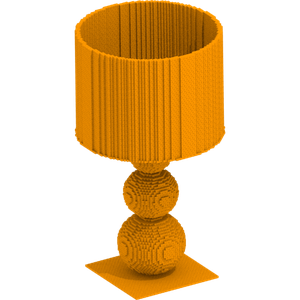
\includegraphics[width=.14\linewidth]{dsp/figs/lamp_0050.png} &
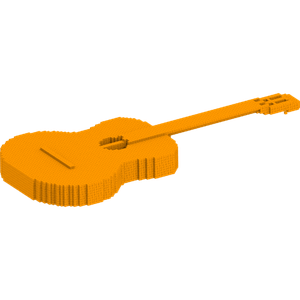
\includegraphics[width=.14\linewidth]{dsp/figs/guitar_0100.png} &
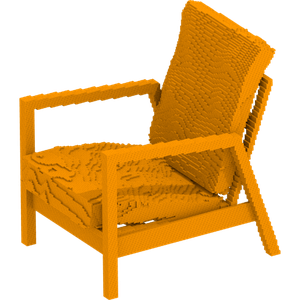
\includegraphics[width=.14\linewidth]{dsp/figs/chair_0011.png} &
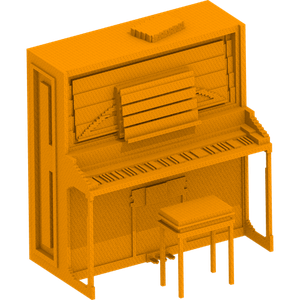
\includegraphics[width=.14\linewidth]{dsp/figs/piano_0050.png} \\
\end{tabular}
    \caption{\small \label{fig:recs} \textbf{Reconstruction from silhouettes without viewpoint noise.}
		3D shapes reconstructed from 8 silhouette images of the same object.
		Viewing angles were sampled uniformly at random.
		Top row using space carving baseline, middle row using the deep image prior, bottom row is ground-truth.
    }
\end{figure*}

For 3D shape reconstruction from silhouette images, we employ the 3D convolutional neural network described as before to generate a voxel grid $V$ where each voxel represents an occupancy value.
The output of the network is then passed to the projection operator $\mathcal{T}_S$ along with a view direction $\phi$.
Given a set of $N$ viewpoints $\bm{\phi} = \{\phi_1, \phi_2, ..., \phi_n\}$ and its associated images $I_{\phi_i}$, our problem is described by the following optimization:
\begin{equation}
    \label{eq:silh}
	\min_{\bm{\theta} \in \mathbb{R}^D} \sum_{i=1}^N||I_{\phi_i} - \mathcal{T}_S(f_{\bm{\theta}}(\bm{\eta}), \phi_i)||_1,
\end{equation}
where $f$ is our neural network and $\bm{\eta}$ its noise input. We solve this minimization using gradient descent and then use $f_{\bm{\theta}}(\bm{\eta})$ to generate our final reconstruction.
The results can be seen in Figure~\ref{fig:binview}.
Even with a small number of silhouette images, our method is able to reconstruct reasonable 3D
shapes.
The viewpoints for this example are chosen by evenly rotating the object along the horizontal axis (e.g. with 4 views, each view is 90 degrees apart; with 8 views, each is 45 degrees apart and so on).
A baseline approach for this problem is space carving, which takes the intersection of all the projected views to generate the occupancy grid.
We show a qualitative comparison with space carving in Figure~\ref{fig:recs}.
Space carving provides reasonable reconstructions for most of the shapes, but some of the objects contain artifacts like creases or even missing parts.
On the other hand, the deep shape prior tends to create overly smooth shapes, which sometimes means removing some parts of the object (chairs in Figure~\ref{fig:recs}) or adding content
where should exist a sharp boundary (lamp in Figure~\ref{fig:recs}).

\paragraph*{View uncertainties.}

In the previous formulation, we assume that the set viewpoints $\bm{\phi}$ corresponds exactly to the observed views.
However, a more realistic scenario is to assume that we are given a set of noisy viewpoint measurements.
In this case, besides estimating the parameters of the network predicting the shape, we are also
looking to estimate viewpoints $\hat{\bm{\phi}}$.
We assume that the noisy viewpoints $\bm{\phi}$ are
sampled independently from $VonMises(\bm{\phi}^*, \kappa)$, where $\kappa$ is the dispersion of the VonMises distribution
with mean $\bm{\phi}^*$ (the ground-truth viewpoints).
This leads to adding an extra term to Equation~\ref{eq:silh} and also optimizing over the predicted viewpoints $\hat{\bm{\phi}}$:
\begin{equation}
    \label{eq:probview}
    \min_{\hat{\bm{\phi}}, \bm{\theta}} \sum_{i=1}^N||I_{\bm{\phi}_i^*} - \mathcal{T}_S(f_{\bm{\theta}}(\bm{\eta}), \bm{\hat\phi}_i)||_1 + \lambda \cos(\bm{\hat{\phi}}_i - \bm\phi_i),
\end{equation}
where $\lambda$ is the weight of the viewpoint regularization term.
We use $\lambda=0.1$ in our experiments.
Notice that our projection operator is fully differentiable with respect to the viewpoint parameters and can be easily
implemented using automatic differentiation packages.


\begin{figure*}[t]
\centering
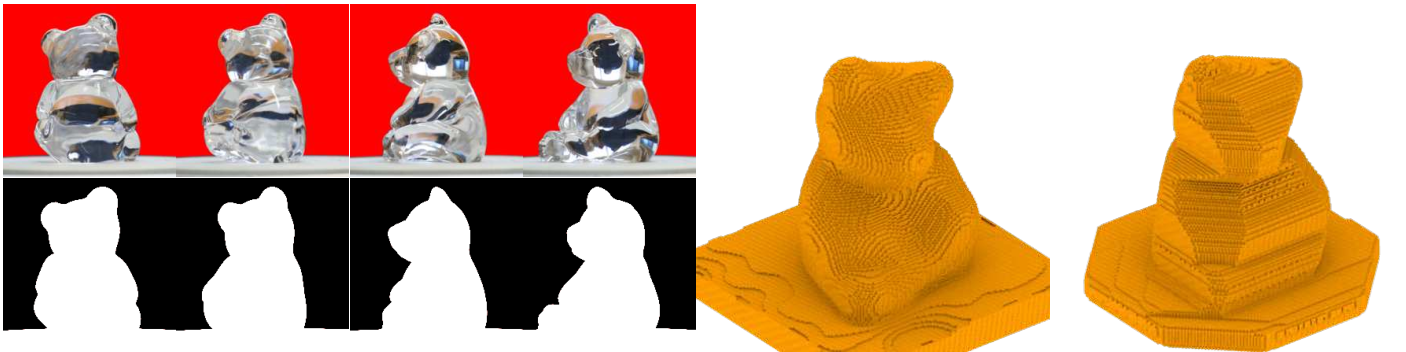
\includegraphics[width=1.0\linewidth]{dsp/figs/realrec.pdf}
\caption{\small \label{fig:panda} \textbf{Shape-from-silhouette reconstruction using captured images.} For this glass object, we photographed 4 views, with 45$^\circ$ angle apart, against a uniform background color. We then applied background-color removal and converted each image to binary silhouette image. The first reconstructed model is the result using our deep prior, whereas the second is the result using the space carving baseline.
    }
    \vspace{10pt}
\end{figure*}


\begingroup
\setlength{\tabcolsep}{2pt} % Default value: 6pt
\renewcommand{\arraystretch}{1.5} % Default value: 1
\begin{table*}
\footnotesize
\centering
{
    \begin{tabular}{l|c|c|c|c|c|c|c|c|c|c|c|c||c}
    & plane & bunny & car & desk & dragon & guitar & lamp & piano & plant & sofa & table & teapot & mean \\
    \hline
    Ours & 0.35 & \textbf{0.88} & \textbf{0.72} & \textbf{0.81} & 0.59 & 0.64 & \textbf{0.62} & \textbf{0.86} & \textbf{0.79} & \textbf{0.78} & \textbf{0.82} & \textbf{0.84} & \textbf{0.72} \\
    Carving & 0.49 & 0.77 & 0.59 & 0.41 & 0.55 & 0.51 & 0.26 & 0.64 & 0.58 & 0.51 & 0.44 & 0.83 & 0.55 \\
    \hline
    Carving$\mathbf{^*}$ & \textbf{0.51} & 0.85 & \textbf{0.72} & 0.50 & \textbf{0.62} & \textbf{0.71} & 0.28 & 0.60 & 0.61 & 0.57 & 0.55 & 0.81 & 0.61 \\
    \end{tabular}
}
\caption{
        \label{tab:rec}
        \textbf{3D reconstruction from silhouettes with uncertain viewpoints.}
        Intersection over union of the reconstructed occupancy from 12 different shapes.
        We randomly sample viewpoints to generate 8 binary images for each shape.
        Those viewpoints are slightly perturbed before being used by the methods, except for the last (Carving$^*$) which corresponds to using space carving
        without noisy viewpoints.
        Our approach significantly outperforms the space carving baseline in all
        scenarios.
}
\end{table*}
\endgroup


\paragraph*{Evaluation}
To evaluate our approach we selected twelve meshes from standard benchmarks.
Three of them are well know 3D shapes (Stanford bunny, dragon and Utah teapot) while the others were selected from 9
different categories of the ModelNet40 dataset~\cite{modelnet}.
We voxelize those shapes filling their interior to generate binary occupancy grids of resolution $108^3$.
Those voxel grids will correspond to our ground-truth data.
Our network generates $128^3$ occupancy grids, but we use data in a smaller resolution to zero-pad the volume and avoid
artifacts in the boundaries.
Next, we randomly sample 8 viewpoints and render a binary image $I_{\phi_i}$ from each sampled view.
Since we want to evaluate the ability of the methods to reconstruct the 3D shape while dealing with view uncertainty,
we sample views $\hat{\bm{\phi}}$ from $VonMises(\bm{\phi}, \kappa)$ and associate them with the corresponding binary images.
We use $\kappa=100$ for all the experiments.
In other words, even though an image $I_\phi$ was rendered from a viewpoint $\phi$, we assign a slightly
perturbed viewpoint $\hat{\phi}$ to this image .
Finally, we use the binary images $I_\phi$ and the perturbed
viewpoints $\hat{\bm{\phi}}$ to reconstruct the 3D shape by minimizing
the objective
described in Equation~\ref{eq:probview}.
This is done through 500 steps of gradient descent.
We compare our approach with a space carving baseline and report the intersection over union of the estimated occupancy grids in Table~\ref{tab:rec}.

Our method outperforms vanilla space carving even when the viewpoints given are not perturbed, which demonstrates the robustness of our method
to viewpoint perturbations.
Figure~\ref{fig:probcomp} shows a qualitative comparison of the reconstructed shapes.
Our approach reconstructs the shapes with high fidelity, preserving details and thin structures.
On the other hand, space carving ends up reconstructing objects with missing parts and
and rough structures as we can observe in Figure~\ref{fig:probcomp}.

\begin{figure*}[t]
\centering
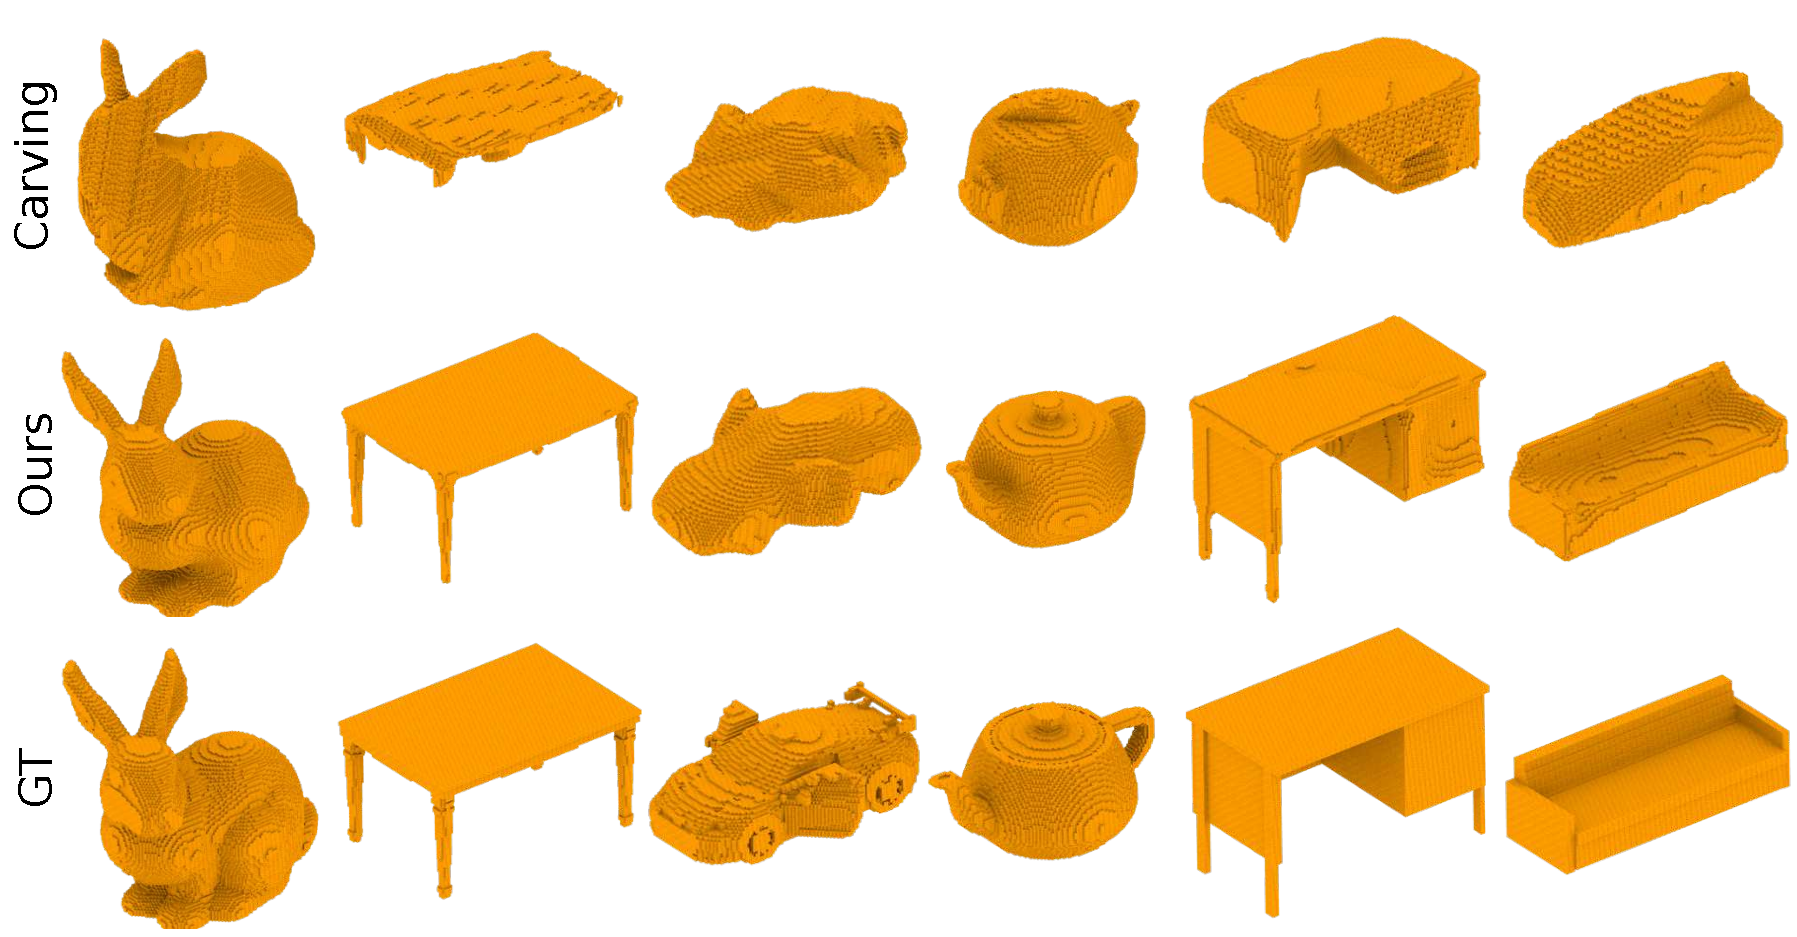
\includegraphics[width=0.9\linewidth]{dsp/figs/probcomp.pdf}
\caption{\small \label{fig:probcomp} \textbf{Shape-from-silhouette reconstruction with perturbed viewpoints.}
Results for the space carving baseline in the first row, our method in the second row, ground-truth shapes in the third row.
Our results are computed minimizing Equation~\ref{eq:probview} through 500 gradient descent steps.
Our method is capable of updating the initial viewpoint parameters and is capable to recover from imprecise viewpoint assignment.
The space carving baseline is not robust to viewpoint perturbations which means it ends up
carving the wrong regions of the volume, leading to poor reconstructions and eliminating
thin object structures.
}
\end{figure*}

\begin{figure}[t]
\centering
\setlength{\tabcolsep}{0pt}
\begin{tabular}{ccccc}
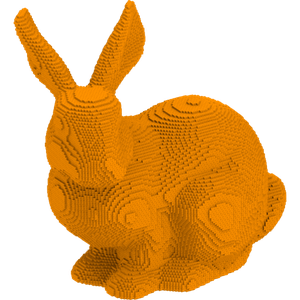
\includegraphics[width=.2\linewidth]{dsp/figs/bunny_deep_4depth_0noise.png} &
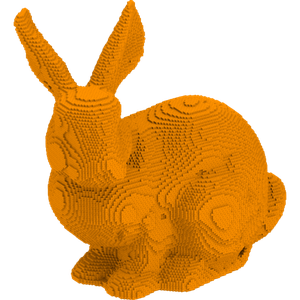
\includegraphics[width=.2\linewidth]{dsp/figs/bunny_deep_4depth_001noise.png} &
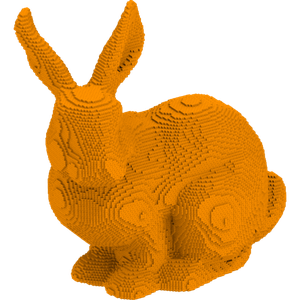
\includegraphics[width=.2\linewidth]{dsp/figs/bunny_deep_4depth_002noise.png} &
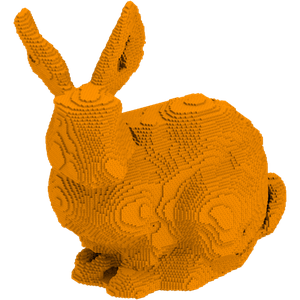
\includegraphics[width=.2\linewidth]{dsp/figs/bunny_deep_4depth_005noise.png} &
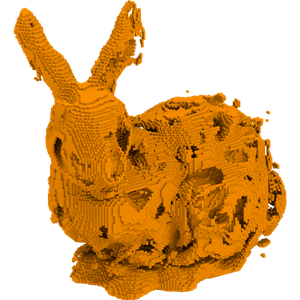
\includegraphics[width=.2\linewidth]{dsp/figs/bunny_deep_4depth_01noise.png} \\
$\sigma=0$ &
$\sigma=0.01$ &
$\sigma=0.02$ &
$\sigma=0.05$ &
$\sigma=0.1$
\end{tabular}
    \caption{\small \label{fig:depthnoise} \textbf{Effect of noise in the reconstruction.}
		3D shape reconstructed from 4 noisy depth images of the same object.
		The variance of the Gaussian noise increases from left to right.
		Shape prior can reconstruct high quality shapes even with considerable amount of noise.
    }
\vspace{0.41in}
\end{figure}

\begin{figure}[t]
\centering
\setlength{\tabcolsep}{0pt}
\begin{tabular}{ccccc}
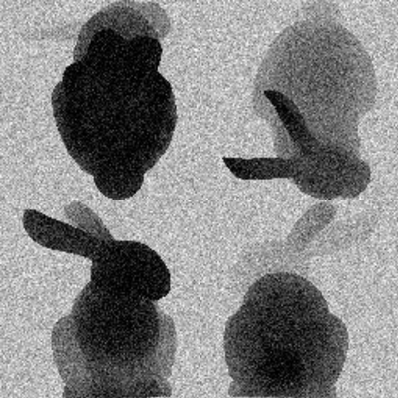
\includegraphics[width=.2\linewidth]{dsp/figs/depthinput.pdf} &
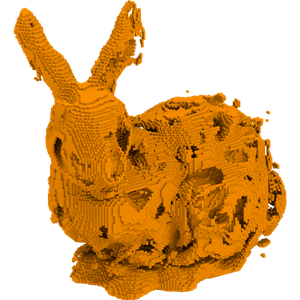
\includegraphics[width=.2\linewidth]{dsp/figs/bunny_deep_4depth_01noise.png} &
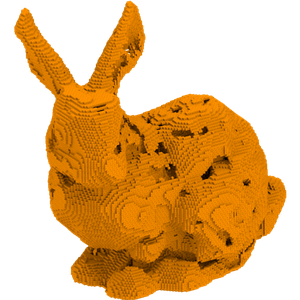
\includegraphics[width=.2\linewidth]{dsp/figs/bunny_deep_8depth_01noise.png} &
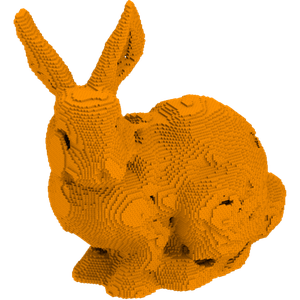
\includegraphics[width=.2\linewidth]{dsp/figs/bunny_deep_16depth_01noise.png} &
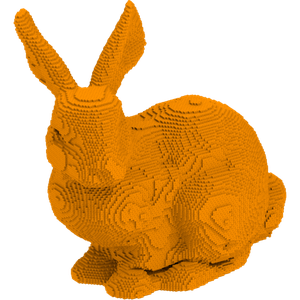
\includegraphics[width=.2\linewidth]{dsp/figs/bunny_deep_32depth_01noise.png}\\
Input&
4 views &
8 views&
16 views&
32 views
\end{tabular}
	\caption{\small \label{fig:depthview} \textbf{Effect of the number of views in the reconstruction from depth images.}
		3D shape reconstructed from very noisy ($\sigma=0.1$) depth images of the same object.
		On the left, example of the input depth images.
		If provided enough views, our method is able to reconstruct high quality shapes even from highly noisy
		inputs.
    }
\end{figure}

\paragraph*{Reconstructions using captured images.} We have also evaluated our method using images captured from a camera. Results are presented in Figure~\ref{fig:panda}. The subject is a glass object, for which we photographed 4 views evenly spaced with 45$^\circ$ horizontal rotation angle apart from each other, against a uniform background color. We then use~\cite{clipmagic} to remove background and convert each image to a binary silhouette image. We compare results using our method with standard visual hull (i.e. space carving). As can be observed, our method leads to smooth reconstructions and the resulting objects look more natural. In contrast, the visual hull results contain artifacts and sharp transitions around changing views, which would require significantly more number of views to eliminate.

\subsection{Shape-from-Depth Images 3D Reconstruction}
The setup for 3D reconstruction from depth images is the same for the binary images except for the use of the projection
$\mathcal{T}_D$ instead of $\mathcal{T}_S$.
All the input depth images have their range scaled to be in $[0, 1]$ using the exponential map in Equation~\eqref{eq:expdepth}.
We analyzed the ability of the method to reconstruct 3D shapes from depth images perturbed by different levels of Gaussian noise
while using 4 views.
Results can be seen in Figure~\ref{fig:depthnoise}.
Additionally, we analyzed the reconstruction quality while varying the number of views.
Results are presented in Figure~\ref{fig:depthview}.
For these experiments, we kept the noise level very high ($\sigma=0.1$).
We notice that even when dealing with very noisy projections, our method is able to reconstruct
high quality shapes if enough views are given.




